\documentclass{tufte-handout}

\usepackage{style}

\begin{document}

\tma{03}

%%%%Question one%%%%
\begin{question}

\qpart
\qsubpart

\underline{Tutor comments:}\par
TMA\textunderscore01 Question 1 was well answered. Through your academic career you will create 
a lot of notes, storing them appropriately is important. 
Part b)  your OpenStudio submission link was incorrect.

\qsubpart

The feedback I received  from the tutor at this point in my studies was very important to me.
I have only ever studied maths modules before this course, and was not fully aware of the importance of making notes,
As a lot of the work is solving problems, and most of the 'notes' are given to us in the handbook, we just have to 
apply them. And the maths I have done so far there is very little need for collaboration, so sharing of working
is limited at this low level of maths.

\qsubpart

I have now started to organise my notes better, not only in this module, but I have invested in a reMarkable
which I use not only to take notes directly onto .PDFs but also I can organised the hand written maths work
and file them in folders, which I have setup to sync with my computer. This means I can easily search for
topics and find my notes quickly.

Word count: 196

\vspace{3cm}

\qpart
\qsubpart

\begin{align*}
\SI{47.5}{\milli\second} &= \SI{47.5e-6}{\second} \\[8pt]
\frac{1}{\SI{47.5e-6}{\second}} &= 21053.2\ldots \\[8pt]
\frac{21053.2\ldots}{1000} &= \SI{21.1}{\kilo\hertz} \\[8pt]
\snote{to 3 s.f.}
\end{align*}

\qsubpart

\begin{align*}
21.053\ldots \times 2.45 &= 51.5\ldots \\[8pt]
\frac{1}{51.5\ldots} &= 0.0194\ldots \\[8pt]
0.0194\ldots \times 1000 &= 19.4\ldots\\[8pt]
&= \SI{19.4}{\micro\second} \\[8pt]
\snote{to 3 s.f.}
\end{align*}

\vspace{3cm}

\qpart

\begin{tabular}{|c|c|}
\hline
Distance/Km & Signal power/W\\
\hline
0 & \SI{2.8e-1}{\watt}\\
\hline
2.35 & \SI{2.8e-2}{\watt} \\
\hline
4.7 & \SI{2.8e-3}{\watt} \\
\hline
7.05 & \SI{2.8e-4}{\watt} \\
\hline
9.4 & \SI{2.8e-5}{\watt} \\
\hline
11.75 & \SI{2.8e-6}{\watt} \\
\hline
\end{tabular}

Hence the signal can tavel \(\SI{11.75}{\kilo\meter}\) before the signal power is
attenuated to \(\SI{2.8}{\micro\watt}\).

\vspace{3cm}

\qpart

Convert 01100010-11101001-11110001-11000111-10101011-01011101 into hexidecimal, first split it into nibbles;

\begin{align*}
0110 &\rightarrow 6\\
0010 &\rightarrow 2\\
1110 &\rightarrow E\\
1001 &\rightarrow 9\\
1111 &\rightarrow F\\
0001 &\rightarrow 1\\
1100 &\rightarrow C\\
0111 &\rightarrow 7\\       
1010 &\rightarrow A\\
1011 &\rightarrow B\\
0101 &\rightarrow 5\\
1101 &\rightarrow D\\
\end{align*}

So the hexadecimal representation is \(62:E9:F1:C7:AB:5D\).

\end{question}

%%%%Question two%%%%
\begin{question}    

    \qpart
    \qsubpart

I would select a class 2 bluetooth device because  with a maxium power output
of \SI{2.5}{\milli\watt} it has a range of about \SI{10}{\meter}, and it is intended
for personal area networks for tings like mobile phones. Whereas class 1 is designed
for business or industrial use with a higher power output of \SI{100}{\milli\watt}
and a range of about \SI{100}{\meter}. And class 3 has a very short range of about
\SI{1}{\meter} with a power output of \SI{1}{\milli\watt}.


    \qsubpart

Both Bluetooth and WIFI are great for short range wireless communication. But 
they differ in their properties and uses. Class 2 bluetooth devices use about 
\(\SI{2.5}{\milli\watt}\)  with a range of about \(\SI{10}{\meter}\) and a bitrate between 
about 1-3 \unit{\mega\bit\per\second}. Making it ideal for accessories like keboards of headphones, where energy and 
hence battery, efficiency matters. 

WIFI on the other hand operates a power output up to \(\SI{100}{\milli\watt}\) and offers a 
range of about \(\SI{80}{\meter}\) with bitrates in the hundreds of \unit{\mega\bit\per\second}. This allows for 
large data intensive tasks such as video streaming of file sharing. But with this comes high 
energy usage it makes WIFI less suitable for battery-powered devices.

Word count: 110

\vspace{3cm}

    \qpart
    \qsubpart

\begin{align*}
\stext{ let \(d_1\) be \(\SI{333}{\metre}\) with a power measurment of \(\SI{27}{\micro\watt}\)}
\stext{ let \(d_2\) be \(\SI{1320}{\metre}\) with a power measurment of \(P\) and using the inverse cube rule}\\
\frac{330}{1320} &= \frac{1}{4}\\[8pt]
\left(\frac{1}{4}\right)^3 &= \frac{1}{64}\\[8pt]
\frac{P}{\SI{27}{\micro\watt}} &= \frac{1}{64}\\[8pt]
P &= \frac{\SI{27}{\micro\watt}}{64}\\[8pt]
&= \SI{0.421875}{\micro\watt}\\[8pt]
&= \SI{4.22e-1}{\micro\watt}\\[8pt]
\snote{to 2 d.p.}\\
\end{align*}

    
    \qsubpart

\begin{align*}
\stext{ let \(d_1\) be \(\SI{330}{\metre}\) with a power measurment of \(\SI{27}{\micro\watt}\)}
\stext{ let \(p_2\) be \(\SI{216}{\nano\watt}\) with a distance of \(d_2\) and using the inverse cube rule}\\
p_2 &= p_1\left( \frac{d_1}{d_2} \right)^3\\[8pt]
d_2 &= d_1\left( \frac{p_1}{p_2} \right)^{\frac{1}{3}}\\[8pt]
&= 330\left( \frac{27\times10^{-6}}{216\times10^{-9}} \right)^{\frac{1}{3}}\\[8pt]
&= 330 \times \left( \frac{1}{8}\times10^{3} \right)^{\frac{1}{3}}\\[8pt]
&= 330 \times (\sqrt[3]{125})\\[8pt]
&= 330 \times 5\\[8pt]
&= \SI{1650}{\metre}\\[8pt]
&= \SI{1.65e3}{\metre}\\
\snote{to 2.d.p.}
\end{align*}

\vspace{3cm}

\qpart
\qsubpart

Accourding to the sampling theorem, if each speech signal has a bandwidth of \(\SI{4}{\kilo\hertz}\),
the minimum sampling rate would be \(\SI{8}{\kilo\hertz}\), which is \( \SI{8000}{\bit\per\second}\).

\qsubpart

\begin{align*}
\stext{The number of bits required to represent 256 quantised levels is }
\log_2(256) &= \SI{8}{\bit}\\[8pt]
\stext{Therefore we needs}
8 + 1 &= 9 \text{ bits per sample, including the 1 bit for TDM sycronisation}\\[8pt]
\stext{using our \(\SI{8000}{\bit\per\second}\)}
9 \times 8000 &= \SI{72000}{\bit\per\second}\\[8pt]
&= \SI{72}{\kilo\bits\per\second}\\
&= \SI{7.2e1}{\kilo\bit\per\second}\\
\snote{to 2 d.p.}
\end{align*}

\qsubpart

\begin{align*}
\stext{Given there are \(48\) users the total bitrate would be }\\
48 \times \SI{7.2e1}{\kilo\bit\per\second}\\ &= \SI{3456}{\kilo\bit\per\second}\\[8pt]
&= \SI{3.46}{\mega\bit\per\second}
\snote{to 2 d.p.}
\end{align*}

\end{question}

%%%%Question three%%%%
\begin{question}
    \qpart
    \qsubpart

https://www.nist.gov/blogs/taking-measure/tale-two-errors-measuring-biometric-algorithms?utm_source=chatgpt.com

    The resource I have chosen is a NIST blog post that explains the trade-off between 
    False Match Rate (FMR) and False Non-Match Rate (FNMR) in biometric identification. 
    Although the article is three years old and some of the statistics may have changed, 
    the overall relationship remains the same. The article succeeds in connecting everyday 
    biometric use, such as unlocking a phone, with high-stakes contexts like crime 
    detection.
    
I found it particularly interesting that as early as the late 1990s, NIST developed 
the detection error trade-off curve, which still remains the sector standard today. 
This shows that the fundamental challenge of balancing false matches with false 
non-matches is not a limitation of computing power but of the nature of biometric 
systems themselves. No matter how advanced or fast algorithms become, the trade-off 
between these two types of error will always exist.

Word count: 140

    \qsubpart

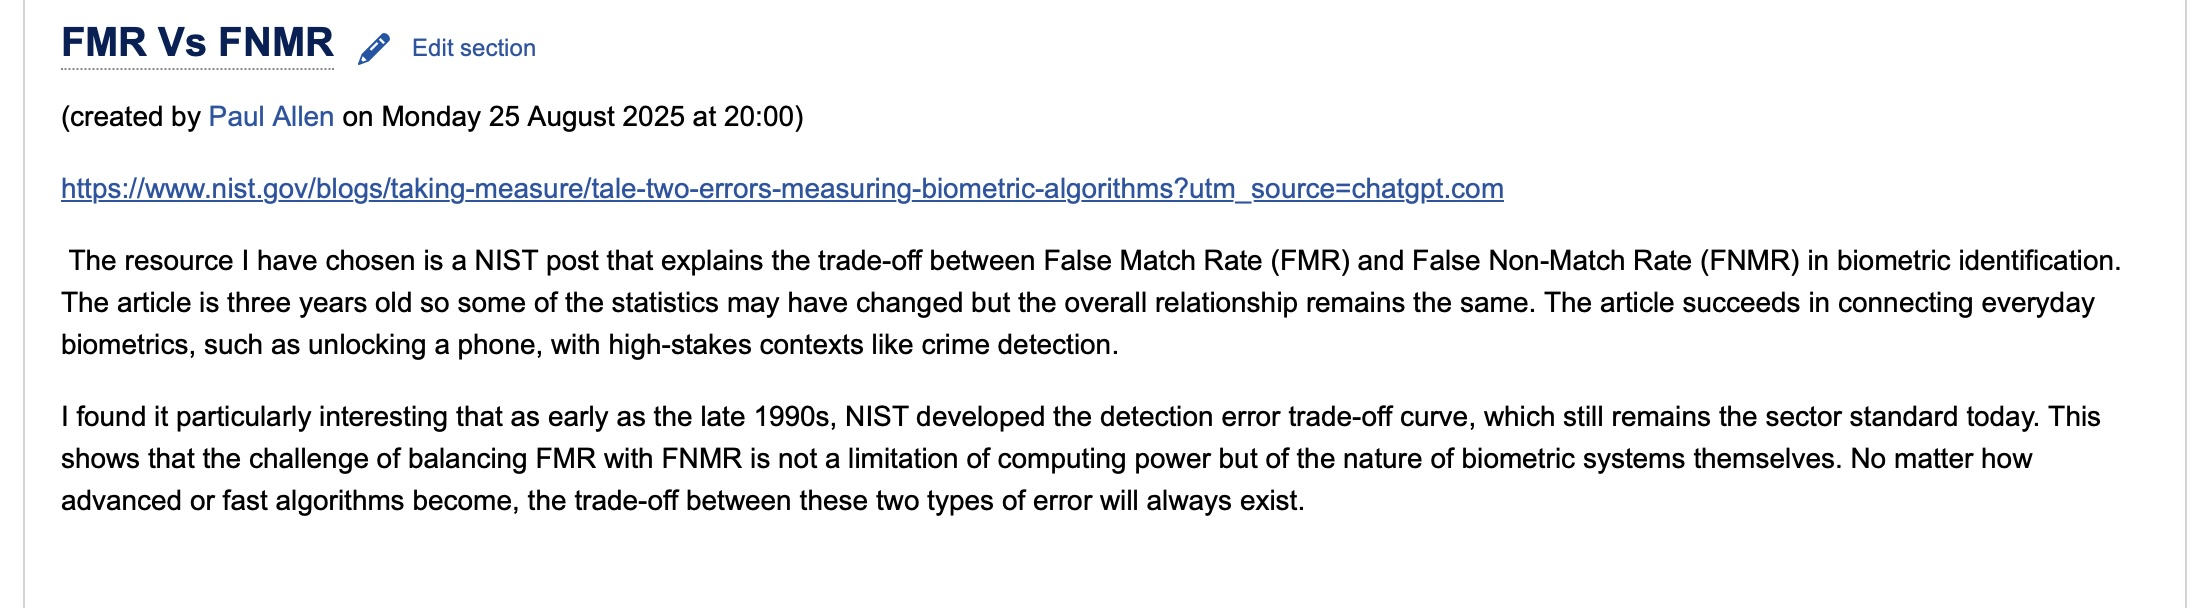
\includegraphics[scale=0.4]{Wiki.jpg}

    \subqpart

    A comment from Paul Allen

I found your resource on digital triage really interesting, especially in showing how 
practices adapted during the pandemic. I agree that the efficiency gained from online tools 
like consultations and messaging is a major benefit, particularly in helping clinicians manage 
time and resources, including the use of non-clinical staff. I also appreciated how the article 
balanced the positives with the challenges, such as accessibility for patients who may struggle
with technology. The article also contains plenty of links to further information making it easy 
to explore the topic in more depth.

Word count: 96

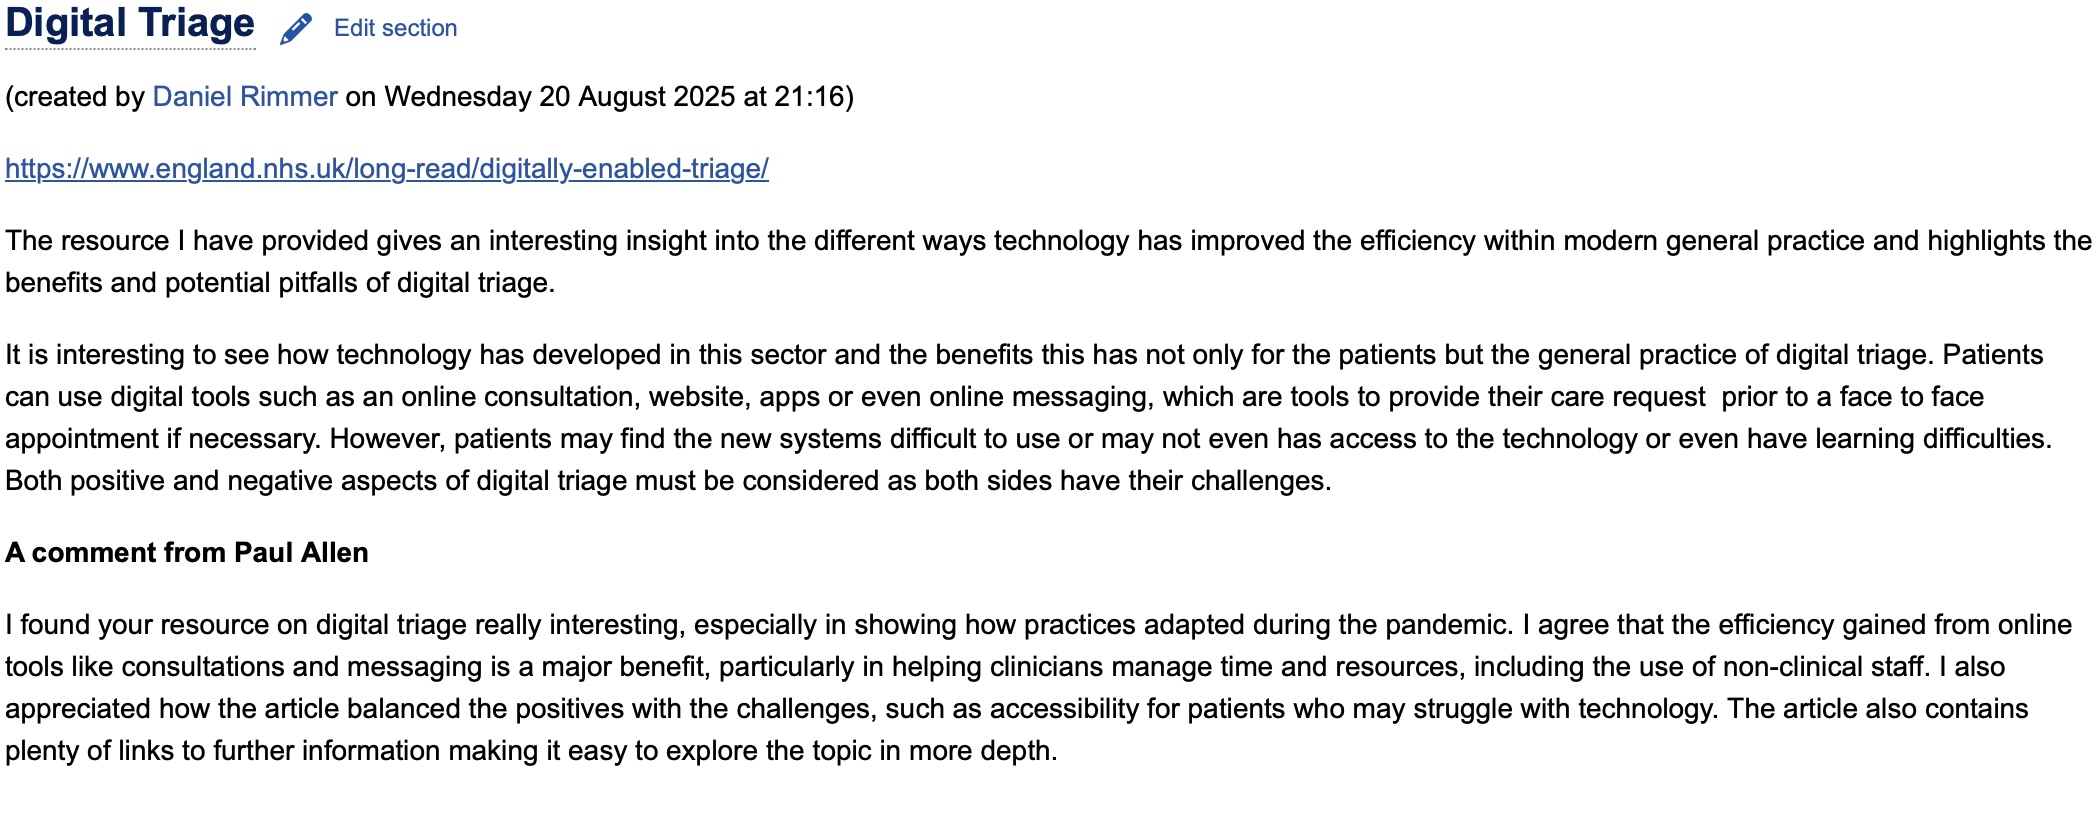
\includegraphics[scale=0.4]{Wiki_comment.jpg}

\qsubpart

When using the tutor group wiki allowed me to reflect on its usability.

In terms of effectiveness: the wiki did as it should; it provides a centralised space for 
student to post resources and text and allows other people to contribute in the form of comments, 
as in our case. I was able to add a section for myself without difficulty, and my comment to another 
student appeared as it should under their post. Showing that it could be used as intended. 

In terms of efficiency: there is a bit more to reflect on. The layout is not immediately intuitive, 
and it took me to read the instructions again use the 'add new section' button, as at first I 
thought this would take me away from the tutorial section. But after re-reading the instructions 
the process was reasonably quick. 

And finally in terms of satisfaction: I found it useful way for students to share resources and 
add comment of their own. If felt collaborative despite the interaction being asynchronous. 
However, the interface itself felt a little dated, in comparison to modern tools like forums of 
chat apps. 

Overall the wiki is effective but could be improved in terms of ease of use and overall 
updating is design elements.

Word count: 208

\vspace{3cm}

\qpart
\qsubpart

The need for accurate age verification online has become an important issue for society as children 
and young people increasingly access social media, gaming platforms and other online services. 
Without effective checks, under-18s can be exposed to harmful content such as violent material, 
online grooming or even the purchase of weapons. For companies, there is also the matter of legal 
compliance, as UK and international regulations place a duty of care on providers to protect young 
users. Reliable age verification helps balance the benefits of digital participation with the 
necessary safeguards.

One leading approach is biometric facial analysis. This works by asking a 
user to provide an image of their face, which is then compared against large datasets of known age 
profiles. The system analyses markers such as bone structure, skin texture and facial ratios to 
estimate whether someone falls above or below a required age threshold. A key advantage is that it 
can be carried out quickly without official documents, which some users may not have or may be 
reluctant to share. Increasingly, the process is being integrated with live images or video to minimise fraud.

Artificial intelligence plays a major role here. AI systems are trained on huge numbers of facial 
images of known ages, which improves the reliability of estimates. The technology can refine 
its predictions by learning subtle patterns invisible to humans. However, this also raises 
questions of fairness, as accuracy may be lower for people from under-represented demographic 
groups if training data lacks diversity.

The accuracy of biometric age verification is improving, with studies suggesting that current 
systems can estimate ages within two to three years. This is sufficient for many purposes, 
such as distinguishing whether a user is under 13 or over 18. Nevertheless, no system is flawless, 
and for higher accuracy some services adopt a layered approach, combining AI-driven facial 
analysis with document checks or parental consent.

\qsubpart

Additional resource:
Ofcom (2024) Children and parents: media use and attitudes report 2024. 
Available at: https://www.ofcom.org.uk/siteassets/resources/documents/research-and-data/media-literacy-research/children/childrens-media-use-and-attitudes-2023/childrens-media-use-and-attitudes-report-2023.pdf 
(Accessed 28 August 2025).

I found this report by searching Google with the terms Ofcom children online report. It was useful because it gave up-to-date statistics on how children in different age groups access media and on which devices. It also highlighted risks faced by young people and parents’ responses, which helped me explain why strong age verification is important.
Word count: 393

\end{question}

\end{document}